\documentclass{article}

\usepackage{amsmath}
\usepackage{amsthm}
\usepackage{amssymb}
\usepackage{mathtools}
\usepackage{bbm}
\usepackage{graphicx}
\usepackage{enumitem}
\usepackage{tikz}
\usepackage{fullpage}

\newtheorem{theorem}{Theorem}

\def\cF{\mathcal{F}}
\def\dR{\mathbb{R}}
\def\mbA{\mathbf{A}}
\def\T{{\mbox{\hspace{-.05em}\scalebox{0.66}{\footnotesize\sffamily T}}}}
\arraycolsep=0.1em

\tikzstyle{vertex}=[circle, inner sep=2pt, draw, ball color=white]
\tikzstyle{labelled vertex}=[circle, inner sep=2pt, draw, ball color=red]

\setlist[itemize]{leftmargin=*, 
     label={\raisebox{.15em}{\footnotesize$\blacktriangleright$}}}

\begin{document}

\section{Installation}

In order to use the Ant building system, both \texttt{ant} and \texttt{cpptasks} have to be installed. For example, in Fedora, these are in the packages \texttt{ant} and \texttt{cpptasks}, respectively. 

Also, the Boost library including headers need to be installed. In Fedora, these are in the package \texttt{boost-devel}.

Compiling all programs in this package is done by a single \texttt{ant} call
in the root directory:

\begin{quote}
\texttt{\$ ant}
\end{quote}

In order to run optimization, Matlab and Cplex need to be installed. For
certifying the solution, you will need Mathematica.




\section{Generating drawings}
There are several separate programs in this package:
\begin{itemize}
\item \textbf{drawingenum}. 
This program enumerates all drawings of the $N\times K$ complete bipartite graph. The program takes two arguments (plus perhaps some options), namely $N$ and $K$.
When used with the \texttt{-vector} option, its output is a list of space-separated numbers. The first line of the output lists $N$ and $K$. All other lines are of the form
\[
\left<id\right>\quad \left<crossing\_count\right> \quad\left<crossings\right>
\]
where $id$ is just a number that counts the number of drawings, 
$crossing\_count$ is the number of crossings that follows, 
and $crossings$ is a list of $crossing\_count$ quadruples $(i, j, k, l)$, each representing a crossing of the edge $a_i b_j$ with the edge $a_k b_l$.
(Here $a_1, \hdots, a_N$ and $b_1, \hdots, b_N$ are the `white' and `black' vertices, respectively, of the bipartite graph.)

Without the \texttt{-vector} option, the output of the program 
is human-readable but less space-efficient.

\item \textbf{canonical}. This program reads the input from DrawingEnum
and calculates the \textit{unlabelled} canonical form of each of the 
drawings returned by DrawingEnum. Each line is of the form
\[
\left<N\right>
\quad\left<K\right>
\quad\left<N_\ell\right>
\quad\left<K_\ell\right>
\quad\left<\rm cr\right> 
\quad\left<crossings\right>
\]
where $crossings$ is the lexicographically smallest vector that can be
obtained by permuting the indices of the white vertices and the black vertices.
Notice that the program only deals with unlabelled flags, so $N_\ell = K_\ell = 0$ for each line in the output.

\item \textbf{generate$\_$drawings}. This program uses DrawingEnum and utils/canonical in combination with the GNU utilities \texttt{sort} and \texttt{uniq}, to determine all isomorphically different drawings. It takes two arguments, $N$ and $K$. The results are saved in the file \texttt{dr$\left<N\right>\left<K\right>$.txt}.
The output format is the same as utils/canonical.
\end{itemize}

\section{Solving the SDP}
Two directories: \texttt{3x3} and \texttt{3x4}

Workflow:
\begin{itemize}
\item Run \texttt{ant generate} in respective directory to generate SDP. 
This generates: matlab files \texttt{parameters.m}, \texttt{crossings.m},
\texttt{CSineq$i$.m}, \texttt{CSmatrix$i$.m}; Mathematica file
\texttt{problemdata.m}.
\item Run \texttt{lp} in Matlab to solve SDP 
\item Run \texttt{savecertificate(wineq)} in Matlab to save certificate (even if lp.m was interrupted)
\item Run \texttt{math $<$ checkcertificate.m} to certify the solution found.
Method: see Section \ref{certification}.
\end{itemize}

\section{Representation of flags}
The flags are partially labelled $N\times K$ bipartite graphs in which we 
store all crossing pairs of edges. 
For example, consider the following (nonexistent) drawing of $K_{3, 4}$ with one crossing:

\begin{center}
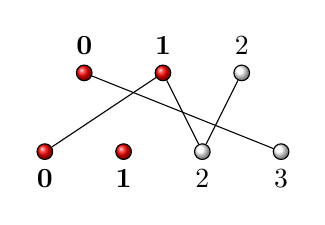
\begin{tikzpicture}
\node[labelled vertex, label=above:$\mathbf{0}$] (a0) at (0.5, 1) {};
\node[labelled vertex, label=above:$\mathbf{1}$] (a1) at (1.5, 1) {};
\node[vertex,          label=above:$2$] (a2) at (2.5, 1) {};

\node[labelled vertex, label=below:$\mathbf{0}$] (b0) at (0, 0) {};
\node[labelled vertex, label=below:$\mathbf{1}$] (b1) at (1, 0) {};
\node[vertex,          label=below:$2$] (b2) at (2, 0) {};
\node[vertex,          label=below:$3$] (b3) at (3, 0) {};

\draw (a0) -- (b3);
\draw (a1) -- (b0); 
\draw (a1) -- (b2); 
\draw (a2) -- (b2); 
\end{tikzpicture}
\end{center}

The flag in this figure has $N=3$ vertices on the top, $K = 4$ on the bottom, $N_\ell = 2$ labelled vertices on the top (marked in red), $K_\ell=2$ labelled vertices on the bottom (marked in red), and ${\rm cr} = 3$ crossings.
So that the labels $0, 1$ on both sides are fixed. The white vertices are unlabelled, i.e., the labels $2, 3$ are meaningless for the flag -- they are only \textit{virtual labels} used for representation in the computer. There are three crossings, namely $a_2b_2$ with $a_0b_3$, $a_1b_2$ with $a_0b_3$, and $a_0b_3$ with $a_1b_0$
(in a purposely unnatural order).
This flag can be represented by the vector
\[
\underbrace{3, 4, 2, 2, 1}_{\mathclap{N, K, N_\ell, K_\ell, {\rm cr}}}, 
\quad \underbrace{2, 2, 0, 3}_{\rm crossing\ 1}
\quad \underbrace{1, 2, 0, 3}_{\rm crossing\ 2}
\quad \underbrace{0, 3, 1, 0}_{\rm crossing\ 3}
\]
Notice that there is some freedom in how we specify this vector. For example, we may switch the first two entries of each crossing with its last two entries. Moreover, we may reorder the crossings. Finally, since the vertices $b_2$ and $b_3$ are unlabelled, we may switch them an obtain the same flag. 
The \textit{canonical form} of a flag is the representation over all permutations of virtual labels of the unlabelled vertices, all permutations of the crossings, and all permutations of the edges within the crossings. The canonical form of the flag above can be constructed by switching labels $2$ and $3$ on the bottom of the graph, which gives
\[
\underbrace{3, 4, 2, 2, 1}_{\mathclap{N, K, N_\ell, K_\ell, {\rm cr}}}, 
\quad \underbrace{2, 3, 0, 2}_{\rm crossing\ 1}
\quad \underbrace{1, 3, 0, 2}_{\rm crossing\ 2}
\quad \underbrace{0, 2, 1, 0}_{\rm crossing\ 3}
\]
and then reordering the crossings and the edges inside them:
\[
\underbrace{3, 4, 2, 2, 1}_{\mathclap{N, K, N_\ell, K_\ell, {\rm cr}}}, \quad 
\quad \underbrace{0, 2, 1, 0}_{\rm crossing\ 3}
\quad \underbrace{0, 2, 1, 3}_{\rm crossing\ 2}
\quad \underbrace{0, 2, 2, 3}_{\rm crossing\ 1}
\]
This canonical form has the property that two flags $F_1$ and $F_2$ have the same canonical form if and only if they are isomorphic.

We construct the set $\cF(N, K; N_\ell, K_\ell)$ as follows. We first generate all drawings of the  $N\times K$ complete bipartite graph in the plane, with the property that no incident edges cross and no two edges cross more than once. For each such drawing, we go through all combinations of ordered subsets of $\{0, \hdots, N-1\}$ (of size $N_\ell$) and ordered subsets of $\{0, \hdots, K-1\}$ (of size $K_\ell$), and label the vertices in these subsets accordingly. We then calculate the canonical form of each of the resulting labelled flags and insert it into the $\cF(N, K; N_\ell, K_\ell)$ if this canonical form has not been seen before. 

For brevity, we will write $\cF(N,K) = \cF(N, K; 0, 0)$.
The flag generation procedure above gives $|\cF(3,3)|=112$, $|\cF(3,4)| = 6393$,
and $|\cF(3,3;3,2)| = 3618$.

%\subsection{Labelled flags}
%Let $\cF(N,K;N_\ell, K_\ell)$ be the set of all $N\times K$ flags that have $N_\ell$ labelled top vertices and $K_\ell$ labelled bottom vertices.
%Internally, these flags are represented as vector as well. Top vertices $0, \hdots, N_\ell-1$ and bottom vertices $0, \hdots, K_\ell-1$ 

\section{The Cauchy-Schwarz matrix}
Fix $N',K',N'_\ell, K'_\ell$ satisfying $0\leq N'_\ell \leq N'\leq N$,\ \  $0\leq K'_\ell \leq K'\leq K$,\ \ $2N_\ell - N' \geq 0$,\ \  and $2K_\ell - K'\geq 0$. These conditions ensure that the number of top and bottom vertices in the product of two elements of $\cF(N',K'; N'_\ell, K'_\ell)$  does not exceed the number of top and bottom of an element in $\cF(N, K)$.

We now construct a matrix $Z(x)$ whose rows and columns are indexed by 
$\cF(N',K'; N'_\ell, K'_\ell)$, and where $x$ is a probability function on $\cF(N, K)$. Each entry corresponding to $F_1, F_2 \in \cF(N',K'; N'_\ell, K'_\ell)$ is given by
\[
\sum_{F\in \cF(N,K)} p(F_1, F_2; F) x(F),
\]
This gives a matrix
We construct the matrix $Z(x)$ by going through each flag $F\in \cF(N,K)$, 
constructing 

\section{Certifying the correctness of the solution\label{certification}}
We are trying to solve the following semidefinite optimization problem:
\[
\begin{array}{ll}
z^* = \min & c^\T x \\
& e^\T x = 1 \\
& Bx \leq b, \\
& A_m(x) \succeq 0, \qquad m=1,\hdots, M.\\
& x \geq 0,
\end{array}
\]
where $x_i$ is the $i$'th flag, $c_i$ is the number of crossings in the $i$'th flag, and $A_m(x)$ is the $m$'th Cauchy-Schwarz matrix. Notice that $A_m(x)$ is linear in $x$, so that we can write
\[
A_m(x) = \sum_{i=1}^n x_i F^{m}_i,
\]
where $F^m_i$ is a constant matrix.
Since $A_m(x)$ is positive semidefinite if and only if $w^\T A_m(x)w\geq 0$ for
all $w\in \dR^{n_m}$, this semidefinite problem may be written 
as a linear optimization problem with infinitely many constraints as follows:
\[
\begin{array}{ll}
z^* = \min & c^\T x \\
& e^\T x = 1 \\
& Bx \leq b, \\
& \displaystyle
\sum_{i=1}^n \left(w^\T F^{m}_iw\right)x_i \geq 0, \mbox{ for all $w\in \dR^{n_m}$, $i=1,\hdots, M$.}\\
& x \geq 0.
\end{array}
\]
Our software generates a finite set $\{w_1, \hdots, w_k\}$ of rational vectors $w$, where vector
$w_j$ corresponds to matrix $A_{m(j)}$. 
Hence, our software solves the linear optimization problem
\[
\begin{array}{ll}
z' = \min & c^\T x \\
& e^\T x = 1 \\
& Bx \leq b, \\
& \displaystyle
\sum_{i=1}^n \left(w_j^\T F^{m(j)}_iw_j\right)x_i \geq 0, \mbox{ for $j =1, \hdots, k$.}\\
& x \geq 0.
\end{array}
\]
Clearly, since the constraints of this latter problem are a subset of infinite set of constraints 
of the original problem, we have that $z' \leq z^*$.  The dual of this problem is
\[
\begin{array}{ll}
z_D = \max & \mu - \nu^\T b\\
& \displaystyle
\mu - \sum_{j=1}^p \nu_j B_j +
 \sum_{j=1}^k \left(w_j^\T F^{m(j)}_i w_j\right) \lambda_j   \leq c^\T_i \\
& \nu \geq 0, \lambda \geq 0, z\mbox{ unrestricted}.
\end{array}
\]
By strong duality, we have $z_D = z' \leq z^*$.
Thus, we have the following theorem:

\begin{theorem}
Let $\lambda \geq 0$ and $\nu\geq 0$. Let
\[
\mu = \min_{j=1, \hdots, n} \left\{c^\T_i + \sum_{j=1}^p \nu_j B_j - \sum_{j=1}^k \lambda_j w_j^\T F^{m(j)}_i w_j\right\}.
\]
Then, $(\lambda, \nu, \mu)$ is a dual feasible solution with objective value
$\mu - \nu^\T b$, and hence $z^* \geq \mu - \nu^\T b$.
\end{theorem}

If
\[
\mu - \sum_{i=1}^p \nu_j B_j + \sum_{j=1}^k \lambda_j w_j^\T F^{m(j)}_i w_j  \leq 
c_j, 
\]
for all $i=1,\hdots, n$, then $(\mu, \nu, \lambda)$ is a dual solution
that certifies that $z^* \geq z' = z_D \geq \alpha$, as required.



\section{Results}

\subsection{3 by 3 case}
We obtain
\[
z^* \geq 1.95245.
\]
This correponds to $0.86775$ times the Zarankiewicz bound

\subsection{3 by 4 case}
We obtain
\[
z^* \geq 4.07257.
\]
This correponds to $0.90501$ times the Zarankiewicz bound


\end{document}
